
\lecture{Introdução ao Gerenciamento de Entrada e Saída (E/S)}{io:intro}

\title{\insertlecture}

\frame{\maketitle}

\part{\insertlecture}

\section{\insertlecture}

\begin{frame}{Entrada e Saída: E/S}  
  \usetikzlibrary{shapes}%add to preambule if the main file does not compile

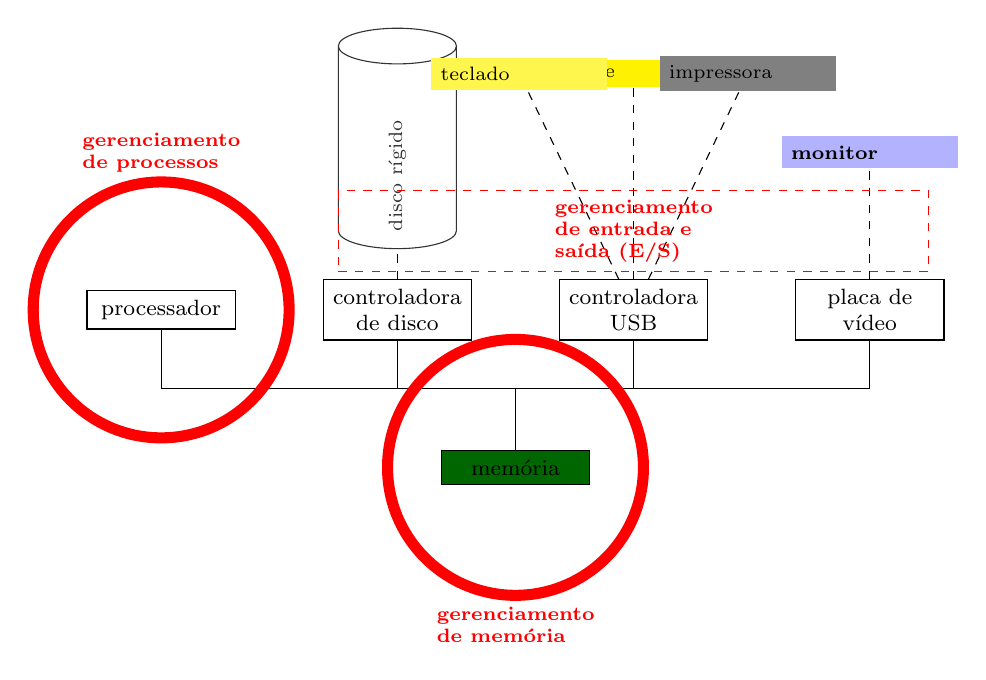
\begin{tikzpicture}[control/.style={text width=1.65cm,align=center,font=\footnotesize,draw},
    every path/.style={draw},device/.style={fill=yellow,font=\scriptsize,minimum width=1cm},
    device connection/.style={dashed},
    disk/.style={black!80,font=\scriptsize,cylinder,minimum width=1.5cm,rotate=90,draw},
    os module/.style={minimum size=3.25cm,circle,red,line width=4,text width=2cm,draw},
    module label/.style={red,font=\bf\scriptsize}]

    \def\dx{3cm}
    \def\dy{2cm}
    
    \node[control] (proc) at (0,0) {processador};
    \node[control] (disk controller) at (\dx,0) {controladora de disco};
    \node[control] (usb controller) at (2*\dx,0) {controladora USB};
    \node[control] (video card) at (3*\dx,0) {placa de vídeo};
    \node[control,fill=green!40!black] (mem) at (1.5*\dx,-\dy) {memória};

    \path (proc) -- +(0,-0.5*\dy) -- +(3*\dx,-0.5*\dy) -- +(video card);
    \path (\dx,-0.5*\dy) -- +(disk controller);
    \path (2*\dx,-0.5*\dy) -- +(usb controller);
    \path (1.5*\dx,-0.5*\dy) -- +(mem);

    \node[disk] (hd) at (\dx,\dy) {disco rígido};
    \path[device connection] (disk controller) -- (hd);

    \node[device] (mouse) [above of=usb controller,yshift=\dy] {mouse};
    \node[device,fill=gray] (printer) [right of=mouse,xshift=.15*\dx] {impressora};
    \node[device,fill=yellow!70] (keyboard) [left of=mouse,xshift=-.15*\dx] {teclado};
    \path[device connection] (usb controller) -- (mouse);
    \path[device connection] (usb controller) -- (printer);
    \path[device connection] (usb controller) -- (keyboard);

    \node[device,fill=blue!30] (monitor) [above of=video card,yshift=.5*\dy] {\bf monitor};
    \path[device connection] (video card) -- (monitor);

    \node<2>[os module] (proc module) at (proc) {};
    \node<2>[module label] [above of=proc module,yshift=.5*\dy] {gerenciamento de processos};

    \node<3>[os module] (mem module) at (mem) {};
    \node<3>[module label] [below of=mem module,yshift=-.5*\dy] {gerenciamento de memória};

    \node<4>[module label,minimum width=7.5cm,dashed,draw] [above of=usb controller] {gerenciamento de entrada e saída (E/S)};
  \end{tikzpicture}

\end{frame}

\begin{frame}{Subsistema de entrada e saída}

  {\small Fonte:~\cite{ufrgs2008}}
  \begin{center}
    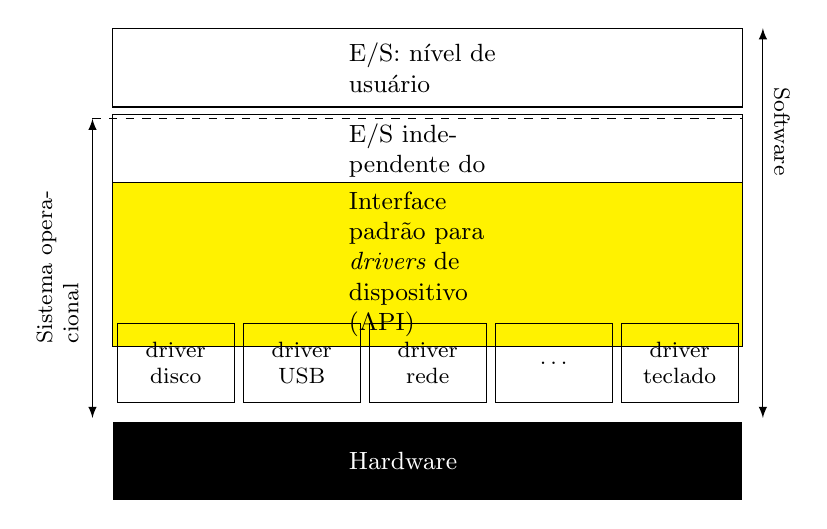
\begin{tikzpicture}[layer/.style={font=\small,minimum height=1cm,minimum width=8cm,draw},
      driver/.style={minimum height=1cm, align=center,font=\footnotesize,text width=1.25cm,draw},
      coda/.style={<->,>=latex}]
    
      \node[layer] (userlevel)  {E/S: nível de usuário};    
      \draw[dashed] (userlevel.west)+(-.25,-.65) -- +(8cm,-.65);
      \draw[coda] (userlevel.west)+(-.25,-.65) -- +(-.25,-4.45cm);
    
      \draw[coda] (userlevel.east)+(.25,.5) -- +(.25,-4.45cm);

      \node[layer] (io0) [below of=userlevel,yshift=-.25cm] {E/S independente do dispositivo};
      \node[layer,fill=yellow] (api) [below of=io0,yshift=-.25cm] {Interface padrão para {\em drivers} de dispositivo (API)};
    
      \foreach \x/\l in {-2/driver disco,-1/driver USB,0/driver rede,1/$\ldots$,2/driver teclado} {
        \node[driver] (driver\x) [below of=api, xshift=1.6*\x cm, yshift=-.25cm] {\l};
      }
      \node[white, fill=black, layer] (hardware) [below of=driver0, yshift=-.25cm] {Hardware};

      \node[rotate=90] [left of=driver-2,yshift=1.5cm,xshift=2.25cm] {Sistema operacional};
      \node [rotate=-90] [right of=io0,yshift=4.5cm,xshift=-1cm] {Software};

    \end{tikzpicture}
  \end{center}

\end{frame}

\begin{frame}{Dispositivos de entrada e saída}

  Além das abstrações de processos, espaços de endereçamento e arquivos,
  os SOs também controlam os dispositivos de E/S para:

  \begin{itemize}
  \item Emitir comandos para dispositivos;
  \item Interceptar interrupções e tratar erros;
  \item Atuar como interface entre os dispositivos e o restante do sistema.
  \end{itemize}

\end{frame}

\begin{frame}{Drivers de dispositivo}{Exemplo: driver de placa de rede}
  \begin{center}  
    
%%% Local Variables: 
%%% mode: latex
%%% TeX-master: "../notes"
%%% End: 


\def\w{2}
\def\h{1.5}
\def\xdelta{1.5}
\def\ydelta{1}
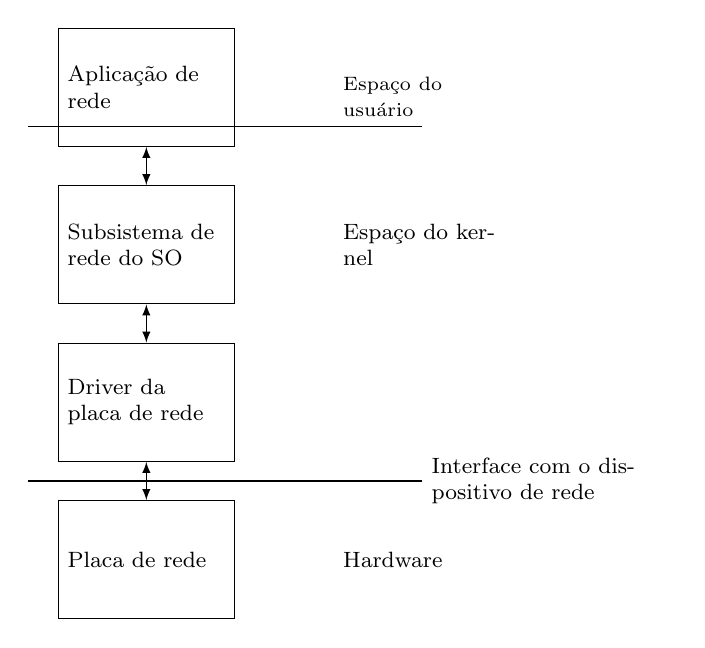
\begin{tikzpicture}
  \tikzset{every node/.style={text width=2cm,font={\footnotesize}},
  module/.style={rectangle,minimum height=1.5cm,draw}}
  \foreach \y/\l in {0/{Aplicação de rede},-2/{Subsistema de rede do
      SO},-4/{Driver da placa de rede},-6/{Placa de rede}} {
    \node[module] (\y) at (0,\y+\h) {\l};
  }
  \foreach \s/\d in {0/-2,-2/-4,-4/-6} {
    \path[<->,>=latex,draw] (\s) -- (\d);
  }

  \draw (-\xdelta,\ydelta) -- (\w+\xdelta,\ydelta) node[above]
  {\scriptsize Espaço
  do usuário};
\node [right of=-2,xshift=25mm] {Espaço do kernel};

  \draw (-\xdelta,-3.5) -- (\w+\xdelta,-3.5) node[text width=3cm,right] {Interface com o
    dispositivo de rede};
  \node [right of=-6,xshift=25mm] {Hardware};
\end{tikzpicture}
  \end{center}
\end{frame}

\begin{frame}{Classificação das camadas de E/S}
  
  \begin{block}<1->{Dispositivos de caracter}
    São dispositivos cujo fluxo de dados ocorre de forma sequencial,
    um byte após o outro.\\
    \smallskip
    Exemplo: teclado, porta serial.
  \end{block}

  \begin{block}<2->{Dispositivos de bloco}
    Os dados são acessados de forma aleatória em pedaços de 
    tamanho fixo chamado blocos.\\
    \smallskip
    Exemplo: Disco rígido, memória flash, disquete, leitor de Blu-ray.    
  \end{block}

  \begin{block}<3>{Dispositivos de rede} Os dados são recebidos e
    transmitidos em pacotes. \\\smallskip
    Exemplo: Interface de rede. 
  \end{block}
  
\end{frame}

\part{Interrupções e DMA}
\frame{\partpage}

\lecture{Interrupções}

\begin{frame}{\insertlecture} 
  \begin{itemize}
  \item<1-> Interrupções permitem que o hardware sinalize o processador;
  \item<2-> Dispositivos de hardware geram interrupções assíncronas com respeito ao 
    relógio ({\it clock}) do processador;
  \item<3> Cada hardware possui um número de interrupção chamado IRQ
    ({\it interrupt request}). Alguns IRQs fixos para PC baseado em
    Intel são listados a seguir:
  \end{itemize}

  \begin{block}<3>{}
    \begin{center}
      \begin{tabular}[h]{c|l}\hline
        \color{red}IRQ &\hfil\color{red} dispositivo \\\hline
        0 & sinal de {\it clock} da placa-mãe \\
        1 & teclado \\
        7 & porta paralela \\
        11 & controlador USB\\\hline
      \end{tabular}
    \end{center}
  \end{block}
  
\end{frame}


\begin{frame}{\insertlecture}
  
  \begin{tikzpicture}[every node/.style={font=\tiny,text centered},
    ctr/.style={text width=1.75cm,draw}, 
    every path/.style={->,>=latex,draw},
    action/.style={text width=2cm,color={gray!70!black}}]

    \node<1-> (K) {\pgfuseimage{keyboard}};
    \node<2->[ctr] (CTRIRQ) [below of=K,yshift=-1cm] {controlador de interrupção};
    \node<3-> (P) [below of=CTRIRQ,yshift=-1cm] {\pgfuseimage{processor}};

    \node<4->[action] (A1) [right of=CTRIRQ, xshift=1.5cm] {processador interrompe o kernel};
    \node<5->[action] (A2) [right of=A1, xshift=1.5cm] {interrupção é manipulada};
    \node<6->[action] (A3) [right of=A2, xshift=1.5cm] {retorna para o código interrompido do kernel};

    \path<2-> (K) -- node[text width=1.2cm,left] {gera interrupção} (CTRIRQ);
    \path<3-> (CTRIRQ) -- (P);
    \path<4-> (P) -- (A1);
    \path<5-> (A1) -- (A2);
    \path<6-> (A2) -- (A3);
  \end{tikzpicture}

\end{frame}

\begin{frame}{Controle das interrupções}

  \begin{itemize}
  \item<1-> As interrupções podem ser desabilitadas para um processador 
    específico;
  \item<2-> Podem ser escolhidas números de IRQs para serem desabilitados 
    pelo SO;
  \item<3> Um mecanismo alternativo à interrupção é o acesso direto à
    memória.
  \end{itemize}
  
\end{frame}

% retirado de Linux Device Drivers
\lecture{Acesso Direto à Memória}

\begin{frame}{\insertlecture}

  \begin{itemize}
  \item<1-> O acesso direto à memória ou DMA ({\it Direct Memory Access})
    é o mecanismo de hardware que permite que periféricos transfiram
    sua E/S diretamente pela memória principal sem envolver o
    processador.
  \item<2-> O uso deste mecanismo a vazão de um dispositivo, pois boa parte 
    da sobrecarga computacional é eliminada.
  \end{itemize}

\end{frame}

\begin{frame}{Processo de transferência de dados, caso 1}{DMA}
  
  No caso 1, o processo pode ser resumido da seguinte forma:
  \begin{enumerate}
  \item<1-> Quando um processo chama uma função para transferência de
    dados, por exemplo {\tt read()} ou {\tt fread()}, o driver aloca
    um {\it buffer} de DMA e instrui o hardware a transferir seus
    dados para este {\it buffer}. O processo é colocado para dormir.
  \item<2-> O hardware escreve os dados no {\it buffer} e lança uma
    interrupção ao término.
  \item<3-> O manipulador de interrupção acessa os dados de entrada,
    responde à interrupção, acorda o processo, que em seguida pode ler
    os dados.
  \end{enumerate}

\end{frame}

%% from LDD pg 441
\begin{frame}{Processo de transferência de dados, caso 1}{DMA}

  O caso 2 ocorre quando o DMA é usado de forma assíncrona. Isto acontece 
  quando um hardware envia dados mesmo quando não há requisição. O processo 
  pode ser resumido da seguinte forma:
  \begin{enumerate}
  \item<1> O hardware lança uma interrupção para anunciar que chegaram
    novos dados.
  \item<2-> O manipulador de interrupção aloca um buffer e comunica ao 
    hardware onde transferir seus dados.
  \item<3-> O dispositivo periférico escreve os dados no {\it buffer}
    e lança outra interrupção ao término.
  \item<4-> O manipulador despacha os dados novos, acorda qualquer processo 
    associado, e se encarrega da liberação da memória utilizada.
  \end{enumerate}

\end{frame}

\lecture{Dispositivos de bloco}

\begin{frame}{\insertlecture}{Introdução}

  \begin{itemize}
  \item Os \alert{\insertlecture} fornecem acesso a dispositivos que
    transferem aleatoreamente blocos de tamanho fixo, tais como disco
    rígido, CD-ROM, DVD-ROM dentre outros.
  \item Os blocos frequentemente possuem o tamanho de \alert{4096
      bytes}, porém, este tamanho pode variar de acordo com a
    arquitetura e sistema de arquivos.
  \end{itemize}

  Drivers eficientes são críticos para performance.

\end{frame}


\begin{frame}{\insertlecture}
  {Conceitos essenciais}
  
  \begin{itemize}
  \item A menor unidade endereçável em um dispositivo de bloco é um \alert{setor}.
  \item O tamanho mais comum do setor é \alert{512} bytes. Porém, alguns dispositivos
    possuem tamanhos diferentes, por exemplo, muitos CD-ROMs possuem setores de 2-KB.
  \item Os blocos são armazenados temporariamente em um zona de memória chamada 
    \alert{\em buffer}, para ajuste entre as diferenças na velocidade de transferência entre
    as camadas dos subsistemas. \\
    \smallskip
    {\small Por exemplo, se a placa de rede suporta envio de blocos 
      de 4-KB, e o SO necessita enviar 64-KB, estes são armazenados no {\em buffer} até
      o término da transmissão.}

  \end{itemize}
        
\end{frame}

\part{Dispositivo de bloco}
\frame{\partpage}

\lecture{Dispositivos de Bloco: Disco Rígido}

\begin{frame}{Busca em disco rígido}{\only<1>{Trilha}\only<2>{Setor}\only<3>{Cabeçote de leitura e escrita}}
  \begin{center}
    
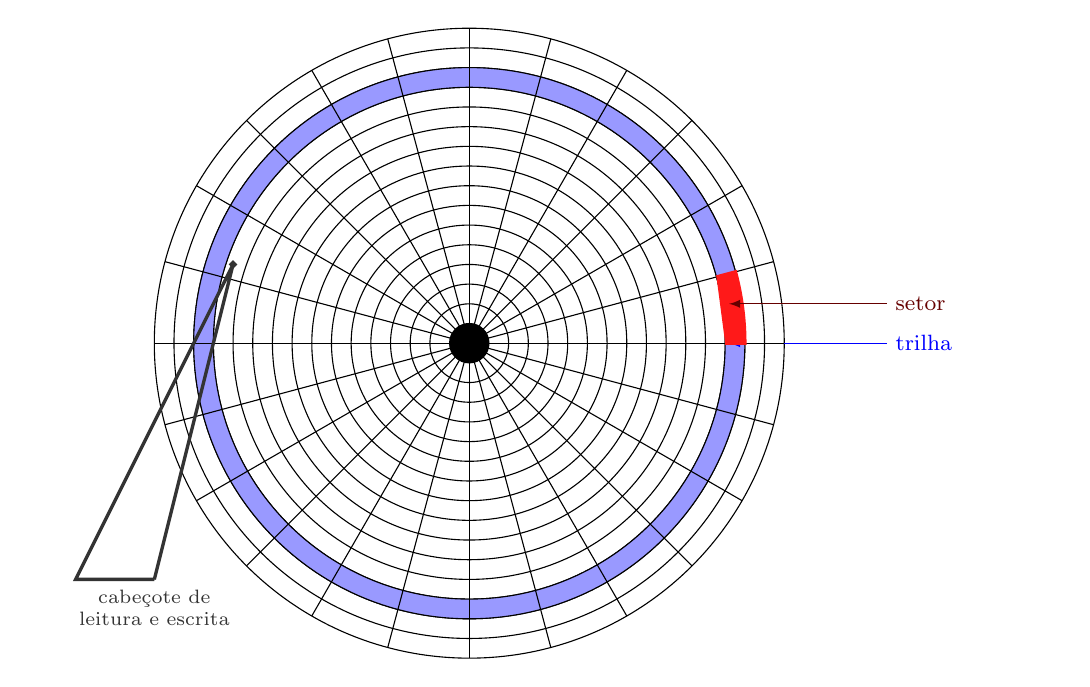
\begin{tikzpicture}\small
  \def\R{4}

  \foreach \d in {0,0.5,1,1.5,...,7} {
    \draw[] (0,0) circle (\R-.5*\d) node (r\d) {};
  }
  \filldraw (0,0) circle (0.25); % AXIS
  \filldraw<1>[even odd rule,fill=blue!40] (0,0) circle (3.5) (0,0) circle (3.25); % TRACK
  \path<1>[blue,draw,<-,>=latex] (3.3,0) -- +(\R/2,0) node[blue,right] {trilha}; % TRACK LABEL
 
  %SECTORS
  \foreach \angle in {0,15,30,...,345}\draw<2-> (0,0) -- +(\angle:\R);
  \filldraw<2>[red!90,very thick] (3.25,0) -- +(.25,0) arc (0:15:3.5) -- +(15:-.25); 
  \path<2>[red!40!black,draw,<-,>=latex] (3.3,0.5) -- +(\R/2,0) node[right] {setor};
 
  %%HEAD
  \path<3>[black!80,draw,very thick] (-4,-3) -- +(1,4) 
  circle (.025) -- +(-1,0) -- (-4,-3) 
  node[font=\scriptsize,text width=3cm,text centered,below] {cabeçote de leitura e escrita}; 

\end{tikzpicture}
  \end{center}
\end{frame}

\lecture{Escalonamento de disco}

\begin{frame}{Escalonamento das requisições de disco}
  
  \begin{itemize}
  \item O \alert{escalonador de disco} gerencia a fila de requisições
    dos dispositivos de bloco, decidindo qual requisição é despachada,
    com o objetivo de maximizar a performance global de E/S do
    sistema.
  \item O escalonadores de disco realizam 2 ações principais sobre as
    requisições para minimizar as buscas:
    \begin{itemize}
    \item \alert{Fusão}: agrupamento de 2 ou mais requisições ao mesmo bloco;
    \item \alert{Ordenação}: classifica as requisições de acordo com
      algum critério.
    \end{itemize}
  \end{itemize}
\end{frame}

\tikzset{plate/.style={}}

\begin{frame}{Algoritmos de escalonamento de disco}{FCFS}
  
  \alert{FCFS}({\em firt-come first-served}): as requisições são
  atendidas conforme a ordem de chegada na fila. Exemplo: 23, 89, 132,
  42, 187. No início o cabeçote está na posição 100.

  \bigskip
  \begin{tikzpicture}[move/.style={->,>=latex,thick,red!60!black, dotted,draw}]
    
    \draw[thick]  (-\textwidth/2,0) node[above] {0} -- (\textwidth/2,0) node[above] {199};
    \node (O) at (0,0) {};
    \node (h100) at (0,.2) {100};
    \node (r23) at (-.77*\textwidth/2,-1*.7) {23};
    \node (r89) at (-.11*\textwidth/2,-2*.7) {89};
    \node (r132) at (.32*\textwidth/2,-3*.7) {132};
    \node (r42) at (-.58*\textwidth/2,-4*.7) {42};
    \node (r187) at (.87*\textwidth/2,-5*.7) {187};

    \path[move] (O) -- (r23);
    \path[move] (r23) -- (r89);
    \path[move] (r89) -- (r132);
    \path[move] (r132) -- (r42);
    \path[move] (r42) -- (r187);

  \end{tikzpicture}

  \pause\footnotesize\hfil  total de trilhas = $77+66+43+90+145 = 421$ trilhas\bigskip

\end{frame}

\begin{frame}{Algoritmos de escalonamento de disco}{SSTS}
  \small
  \alert{SSTF} ({\em shortest seek time first}): as requisições
  são atendidas de acordo com o menor tempo de acesso, e são
  reordenadas constantemente, para levar em conta a posição atual do
  cabeçote, privilegiando os setores mais próximos à posição
  corrente na reordenação da fila de requisições.

  \begin{tikzpicture}[move/.style={->,>=latex,thick,red!60!black, dotted,draw}]
    
    \draw[thick]  (-\textwidth/2,0) node[above] {0} -- (\textwidth/2,0) node[above] {199};
    \node (O) at (0,0) {};
    \node (h100) at (0,.2) {100};
    \node (r89) at (-.11*\textwidth/2,-1*.7) {89};
    \node (r132) at (.32*\textwidth/2,-2*.7) {132};
    \node (r187) at (.87*\textwidth/2,-3*.7) {187};
    \node (r42) at (-.58*\textwidth/2,-4*.7) {42};
    \node (r23) at (-.77*\textwidth/2,-5*.7) {23};

    \path[move] (O) -- (r89);
    \path[move] (r89) -- (r132);
    \path[move] (r132) -- (r187);
    \path[move] (r187) -- (r42);
    \path[move] (r42) -- (r23);

  \end{tikzpicture}

  \bigskip

  \only<2>{\footnotesize\hfil total de trilhas =
    $11+43+55+145+19 = 273$ trilhas}

  \only<3>{\color{red}\small Desvantagem: Suscetível à postergação
    indefinida ({\em starvation}).}
\end{frame}
  
\begin{frame}{Algoritmos de escalonamento de disco}{SCAN}
  \footnotesize
  \alert{SCAN}: é uma variação do SSTF que se diferencia por
  adotar um sentido de varredura preferencial, como por exemplo do
  mais interno para o mais externo. Ao atingir o mais interno,
  inverte-se o sentido e novas requisições no sentido contrário são
  atendidas na próxima varredura. 
  
  \begin{tikzpicture}[move/.style={->,>=latex,thick,red!60!black, dotted,draw}]
    
    \draw[thick]  (-\textwidth/2,0) node[above] {0} -- (\textwidth/2,0) node[above] {199};
    \node (O) at (0,0) {};
    \node (h100) at (0,.2) {100};
    \node (r89) at (-.11*\textwidth/2,-1*.6) {89};
    \node (r42) at (-.58*\textwidth/2,-2*.6) {42};
    \node (r23) at (-.77*\textwidth/2,-3*.6) {23};
    \node (left) at (-\textwidth/2,-4*.6) {0};
    \node (r132) at (.32*\textwidth/2,-5*.6) {132};
    \node (r187) at (.87*\textwidth/2,-6*.6) {187};

    \path[move] (O) -- (r89);
    \path[move] (r89) -- (r42);
    \path[move] (r42) -- (r23);
    \path[move] (r23) -- (left);
    \path[move] (left) -- (r132);
    \path[move] (r132) -- (r187);
  \end{tikzpicture}
  
  \bigskip

  \only<2>{\footnotesize\hfil total de trilhas =
    $11+47+19+23+132+55 = 287$ trilhas}

  \only<3>{Também é conhecido como algoritmo do \alert{elevador}.}

\end{frame}

\begin{frame}{Algoritmos de escalonamento de disco}{C-SCAN}

  \alert{C-SCAN}: variação do SCAN que se diferencia por adotar
  o sistema de varredura em somente uma direção. Por exemplo, se o
  cabeçote atingir o cilindro mais interno, é então reposicionado
  no cilindro mais externo e a varredura é realizada novamente.

  \begin{tikzpicture}[move/.style={->,>=latex,thick,red!60!black, dotted,draw}]
    
    \draw[thick]  (-\textwidth/2,0) node[above] {0} -- (\textwidth/2,0) node[above] {199};
    \node (O) at (0,0) {};
    \node (h100) at (0,.2) {100};
    \node (r89) at (-.11*\textwidth/2,-1*.5) {89};
    \node (r42) at (-.58*\textwidth/2,-2*.5) {42};
    \node (r23) at (-.77*\textwidth/2,-3*.5) {23};
    \node (left) at (-\textwidth/2,-4*.5) {0};
    \node (right) at (\textwidth/2,-5*.5) {199};
    \node (r187) at (.807*\textwidth/2,-6*.5) {187};
    \node (r132) at (.32*\textwidth/2,-7*.5) {132};

    \path[move] (O) -- (r89);
    \path[move] (r89) -- (r42);
    \path[move] (r42) -- (r23);
    \path[move] (r23) -- (left);
    \path[move] (left) -- (right);
    \path[move] (right) -- (r187);
    \path[move] (r187) -- (r132);
  \end{tikzpicture}

  \bigskip

  \only<2>{\footnotesize\hfil total de trilhas =
    $11+47+19+23+199+12+55 = 366$ trilhas}

\end{frame}


\begin{frame}
  
  \begin{thebibliography}{5}
  \bibitem[Oliveira, 2008]{ufrgs2008}
    {\em Sistemas Operacionais}.
    \newblock Rômulo Silva de Oliveira, Alexandre da Silva Carissimi e 
    Simão Sirineo Roscani.
    \newblock Editora Bookman, 2008.
  
  \bibitem[LKD3]{lkd3} 
    {\em Linux Kernel Development}.
    \newblock Robert Love.
    \newblock Addison Wesley, 3rd edition, 2010.

  \bibitem[LDD3]{ldd3} 
    {\em Linux Device Drivers}.
    \newblock Jonathan Corbet, Alessandro Rubini, Greg Kroah-Hartman.
    \newblock O'Reilly, 3rd edition, 2010.

  \bibitem[WAGmob]{wagmob} 
    {\em Operating System 101}.
    \newblock WAGmob.

  \bibitem[Garrido, 2008]{garrido2008}
    {\em Principles of Modern Operating Systems}.
    \newblock José M.\ Garrido, Richard Schlesinger.
    \newblock Jones and Bartlett Publishers, 2008.

  \end{thebibliography}

\end{frame}


\lecture{Exercício de Escalonamento de E/S}{io:exercise}

\begin{frame}{Exercício}

  \begin{enumerate}
  \item Dada as seguintes sequências de requisições para um 
    disco com $100$ trilhas:
    \begin{center}
      $44, 20, 95, 4, 50, 52, 47, 61, 87, 25$,
    \end{center}
    onde a posição atual dos cabeçotes é $50$, calcule a deslocamento
    de dos cabeçotes para atender às requisições utilizando os
    seguintes algoritmos de escalonamento de E/S:
    \begin{enumerate}
    \item FCFS;
    \item SSTF;
    \item SCAN;
    \item C-SCAN.
    \end{enumerate}
  \end{enumerate}
  
\end{frame}

